\documentclass{beamer}
\mode<presentation>
\usepackage{amsmath}
\usepackage{amssymb}
%\usepackage{advdate}
\usepackage{adjustbox}
\usepackage{subcaption}
\usepackage{enumitem}
\usepackage{multicol}
\usepackage{mathtools}
\usepackage{listings}
\usepackage{hyperref}
\usepackage{listings}
\usepackage{url}
\usepackage{hyperref}
\def\UrlBreaks{\do\/\do-}
\usetheme{Boadilla}
\usecolortheme{lily}
\setbeamertemplate{footline}
{
  \leavevmode%
  \hbox{%
  \begin{beamercolorbox}[wd=\paperwidth,ht=2.25ex,dp=1ex,right]{author in head/foot}%
    \insertframenumber{} / \inserttotalframenumber\hspace*{2ex} 
  \end{beamercolorbox}}%
  \vskip0pt%
}
\setbeamertemplate{navigation symbols}{}

\providecommand{\nCr}[2]{\,^{#1}C_{#2}} % nCr
\providecommand{\nPr}[2]{\,^{#1}P_{#2}} % nPr
\providecommand{\mbf}{\mathbf}
\providecommand{\pr}[1]{\ensuremath{\Pr\left(#1\right)}}
\providecommand{\qfunc}[1]{\ensuremath{Q\left(#1\right)}}
\providecommand{\sbrak}[1]{\ensuremath{{}\left[#1\right]}}
\providecommand{\lsbrak}[1]{\ensuremath{{}\left[#1\right.}}
\providecommand{\rsbrak}[1]{\ensuremath{{}\left.#1\right]}}
\providecommand{\brak}[1]{\ensuremath{\left(#1\right)}}
\providecommand{\lbrak}[1]{\ensuremath{\left(#1\right.}}
\providecommand{\rbrak}[1]{\ensuremath{\left.#1\right)}}
\providecommand{\cbrak}[1]{\ensuremath{\left\{#1\right\}}}
\providecommand{\lcbrak}[1]{\ensuremath{\left\{#1\right.}}
\providecommand{\rcbrak}[1]{\ensuremath{\left.#1\right\}}}
\providecommand{\abs}[1]{\ensuremath{\left\vert#1\right\vert}}
\providecommand{\mean}[1]{\ensuremath{E\left[ #1 \right]}}
\theoremstyle{remark}
\newtheorem{rem}{Remark}
\newcommand{\sgn}{\mathop{\mathrm{sgn}}}
\providecommand{\res}[1]{\Res\displaylimits_{#1}} 
\providecommand{\norm}[1]{\lVert#1\rVert}
\providecommand{\mtx}[1]{\mathbf{#1}}
\providecommand{\fourier}{\overset{\mathcal{F}}{ \rightleftharpoons}}
%\providecommand{\hilbert}{\overset{\mathcal{H}}{ \rightleftharpoons}}
\providecommand{\system}{\overset{\mathcal{H}}{ \longleftrightarrow}}
	%\newcommand{\solution}[2]{\textbf{Solution:}{#1}}
%\newcommand{\solution}{\noindent \textbf{Solution: }}
\providecommand{\dec}[2]{\ensuremath{\overset{#1}{\underset{#2}{\gtrless}}}}
\newcommand{\myvec}[1]{\ensuremath{\begin{pmatrix}#1\end{pmatrix}}}
\let\vec\mathbf

\lstset{
%language=C,
frame=single, 
breaklines=true,
columns=fullflexible
}

\numberwithin{equation}{section}

\title{Matgeo Presentation}
\author{Ronit Ranjan \\ AI24BTECH11028\\IIT Hyderabad.}

\date{\today} 
\begin{document}

\begin{frame}
\titlepage
\end{frame}

\section*{Outline}
\begin{frame}
\tableofcontents
\end{frame}
\section{Problem}
\begin{frame}
\frametitle{Problem Statement}

Find the coordinates of the point which divides the line segement joining the points (-2, 3, 5) and (1, -4, 6) in the ratio\\
i) 2:3 internally\\
ii) 2:3 externally
\end{frame}


\section{Solution}
\subsection{Internal Division}
\begin{frame}
\frametitle{Internal Division}

For internal divison we have,
\begin{align}
    D = \frac{kC + B}{k + 1}
\end{align}
\begin{table}[h]
    \centering
    \begin{tabular}{|c|c|}
\hline
\textbf{Variables} & \textbf{Values}\\
\hline
\textbf{B} & $\myvec{-2\\3\\5}$\\
\hline
\textbf{C} & $\myvec{1\\-4\\6}$\\
\hline
\textbf{k} & $\frac{2}{3}$\\
\hline
\end{tabular}

\end{table}
\end{frame}
\subsection{Changing everything to Matrix form}
\begin{frame}
\frametitle{Changing everything to Matrix form}
Now, Putting values in the equation we get,
\begin{align}
D = \frac{\frac{2}{3}
 \myvec{
   1
   \\
   -4
   \\
   6
 }
 +
 \myvec{
   -2
   \\
   3 
   \\
   5
 }}{\frac{2}{3}+1}
 \\
 D = \frac{
  \myvec{
  \frac{-4}{3}
  \\
  \frac{1}{3}
  \\
  9
  }
  }{\frac{5}{3}}
  \\
D = 
 \myvec{
  \frac{-4}{5}
  \\
  \frac{1}{5}
  \\
  \frac{27}{5}
 }
 \end{align}
 
So, the point which divides the line segement joining the points \brak{2, 3, 5} and \brak{1, -4, 6} is \brak{\frac{-4}{5}, \frac{1}{5}, \frac{27}{5}}

\end{frame}
\subsection{External Division}
\begin{frame}
\frametitle{External Division}
For external divison we have,
\begin{align}
    D = \frac{kC - B}{k - 1}
\end{align}
\end{frame}

\subsection{Changing everything to matrix form}
\begin{frame}
\frametitle{Changing everything to matrix form}
Now, Putting values in the equation we get,
\begin{align}
D = \frac{\frac{2}{3}
 \myvec{
   1
   \\
   -4
   \\
   6
 }
 -
 \myvec{
   -2
   \\
   3 
   \\
   5
 }}{\frac{2}{3}-1}
 \\
 D = \frac{
  \myvec{
  \frac{8}{3}
  \\
  \frac{-35}{3}
  \\
  -1
  }
  }{\frac{-1}{3}}
  \\
D = 
 \myvec{
  -8
  \\
  17
  \\
  3
 }
 \end{align}
 So, the point which divides the line segement joining the points \brak{2, 3, 5} and \brak{1, -4, 6} is \brak{-8, 17, 3}
    
\end{frame}


\section{Codes}
\begin{frame}[fragile]
\frametitle{Codes}
For internal division:
\resizebox{\textwidth}{!}{\fbox{\url{https://github.com/igiamronit/EE1030/blob/main/matgeo assignment1/codes/Internal Divison/data.c}}}
For external divsion:
\resizebox{\textwidth}{!}{\fbox{\url{https://github.com/igiamronit/EE1030/blob/main/matgeo assignment1/codes/External Divison/data.c}}}





\end{frame}

\section{Figures}
\subsection{Plot for internal divison}
\begin{frame}
\frametitle{Plot for internal divison}
\begin{figure}[hbt!]
		\centering
		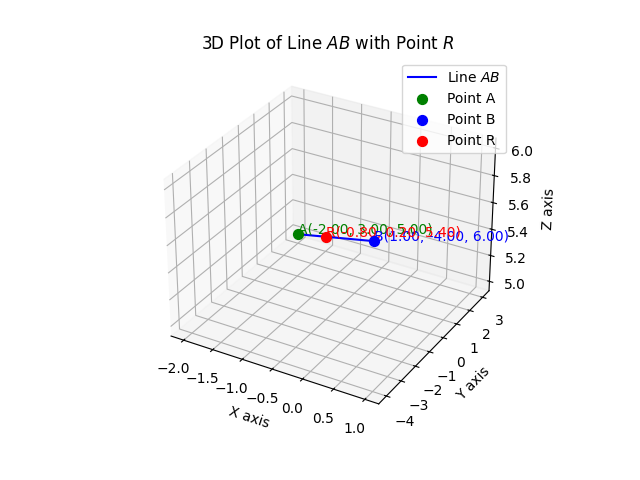
\includegraphics[width=0.8\linewidth]{plots/plot1.png}

	\end{figure}
\end{frame}

\subsection{Plot for external divison}
\begin{frame}
\frametitle{Plot for external divison}
\begin{figure}[hbt!]
		\centering
		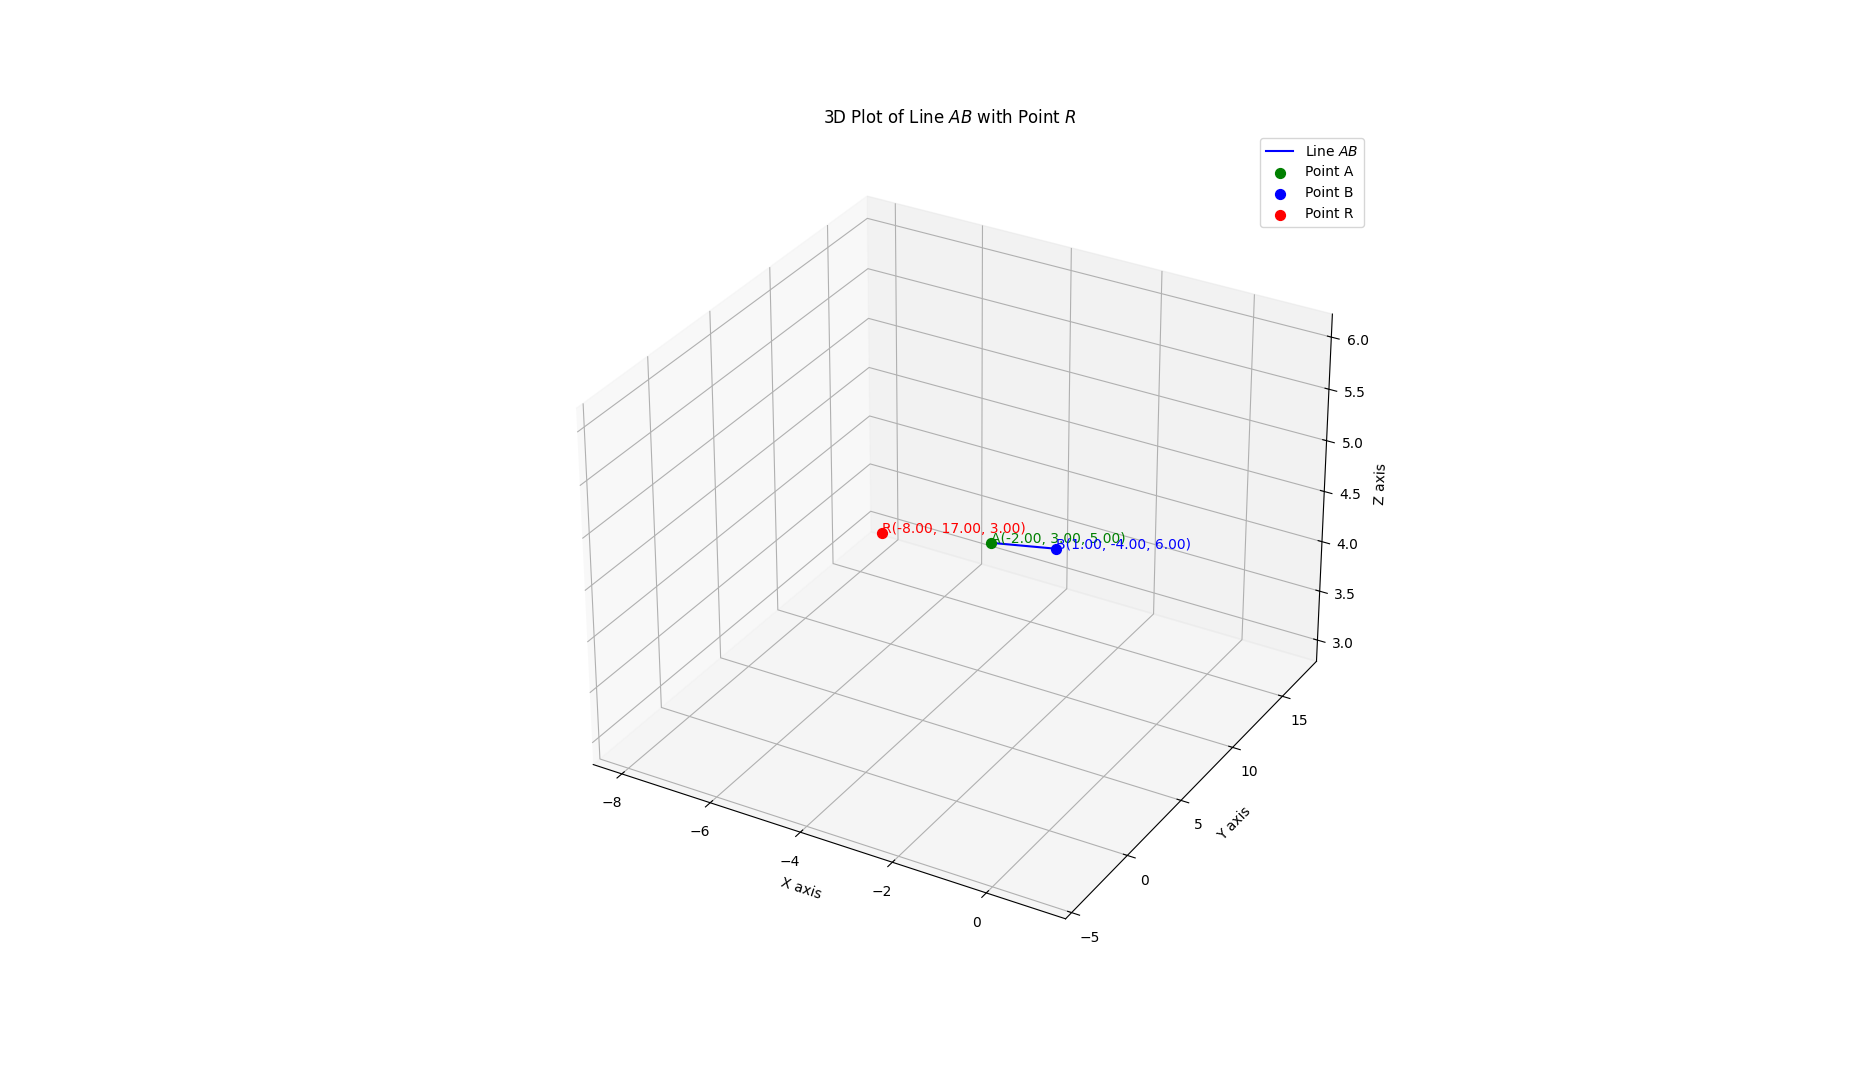
\includegraphics[width=0.9\linewidth]{plots/plot2.png}

	\end{figure}


\end{frame}





\end{document}
